\begin{savequote}[75mm]
The man who is swimming against the stream knows the strength of it.
\qauthor{Woodrow Wilson}
\end{savequote}

\chapter{Stream Processing}
Steams are older then computers so it is not a big surprice that streams
and the processing of them isn't a absolutly new topic in the computer science world.
Historically there are techniques like \textbf{logging} or in the domain driven development area there is \textbf{event sourcing},
which are very similar to streaming processing.
But they have not always been such an important deal like they is today with the with the unbelievable amount of data.
Antecedent to handle this streams was an event driven way and do analytics after storing the data.\\

\newpage

\section{Frozen yogurt}
Let me explain the \textit{old} event driven way with a small example.\\
Imagine a factory which produces frozen yogurt in different flavors.
They weigh and register every cup of yogurt at the end of the assembly line.\\

\begin{figure}[H]
\centering
\captionsetup{justification=centering}
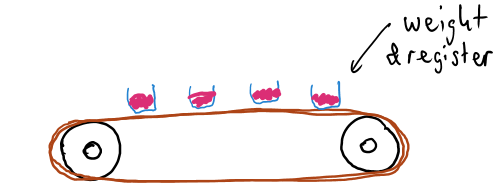
\includegraphics[width=0.5\textwidth]{images/cups.png}
\caption[Frozen yogurt assembly line]{frozen yogurt assembly line}
\end{figure}

\subsection{Common architecture}
The factory has sensors which weight the cups and this weights are sent to a server.
The server handles the request and stores the frozen yogurt with his weight in the database.
for analytic tasks there is a web application. If you are now interested in the total amount of produced cups.
You can simply open the browser go to the analytic page.
This starts a request to the server and the server will call the database with a quey like "select count(*) from frozen\_yogurt".
After the quey is executed you will get the result from the server and have the aggregated nummer on your screen.\\
(This is more or less a default example of a Three-tier architecture)

\begin{figure}[H]
\centering
\captionsetup{justification=centering}
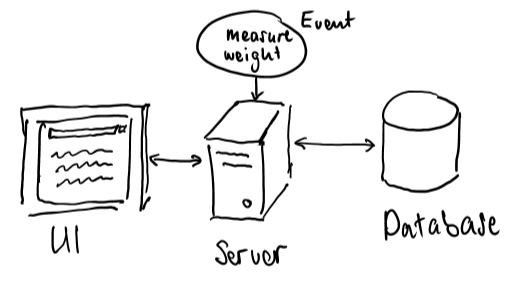
\includegraphics[width=0.6\textwidth]{images/three_tier.png}
\caption[Three-tier architecture]{Three-tier architecture}
\end{figure}

\newpage

Now the owner of the factory does a very good business and they are able to expand the production.
And with this expansion they also add a lot more of sensors to the assembly line like, a temperature sensor,
optical recognition to check if the cups are always full and a lot more.\\
The requirements of the system are also updated the owner want to have statistic about the production all the time
and want's immediately notifications if for example the temperature is to high.\\
These new requirements leads to new challenges in the architecutre of the system and are hard to implement with the
current state and the enormus data produced by the all sensors.

\begin{figure}[H]
\centering
\captionsetup{justification=centering}
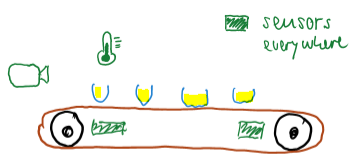
\includegraphics[width=0.6\textwidth]{images/sensors.png}
\caption[sensors everywhere]{sensors everywhere}
\end{figure}

\subsection{Streaming architecture}
A good way to handle this new requirements is to continuous aggregate and filter the stream of data before it is stored in the database.
For this purpose there has grown up a lot of new techniques and frameworks during the last few years.

\begin{figure}[H]
\centering
\captionsetup{justification=centering}
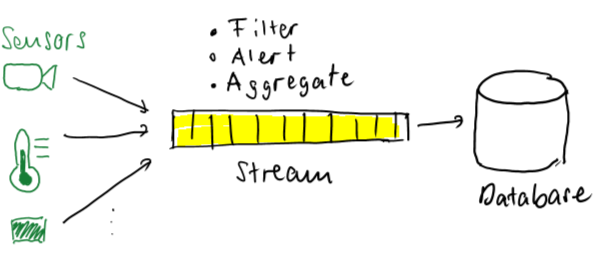
\includegraphics[width=0.7\textwidth]{images/stream.png}
\caption[streaming architecture]{streaming architecture}
\end{figure}

\newpage

\subsection{Conclusion}
The new streaming architecture of the frozen yogurt factory has got a lot of advantages but also has to handle some big difficulties.
Now it is possible to get very fast access to production statistics, deal with the huge amount of data and throw alerts in real time.
It's also helpfull in the developers perspective, because you can add several consumer to the stream.
Normaly this stream is immutable if you use a technologie like kafka, which has the advantage that there aren't concurrency problems anymore.
Thus the requirements in such real time stream processing systems are ambitious and we will face them in the next section.

\newpage

\section{Eight Rules For Stream Procesing}
In the paper "The 8 Requirements of Real-Time Stream Processing" Michael Stonebraker, Uğur Çetintemel and Stan Zdonik
bring their thoughts about real-time stream processing together and write it down. It faces the fundamental ideas of stream processing
and sums them up in eight rules which every stream processing engine should require.
This allows us to measure and compare different technologies.
Thus leads me to take a closer look at these rules and add my reflection to them.

\subsection{Rule 1: Keep the Data Moving}
\textit{The first requirement for a real-time stream processing
        system is to process messages “in-stream”, without any
        requirement to store them to perform any operation or
        sequence of operations. Ideally the system should also use
        an active (i.e., non-polling) processing model.}

\medskip
This is also for me a very important point. The stream processing should not slow down the "in-stream".
How can this target be reached? The paper says be aware of expensive storage operation.
But I could imagine that this question depends most on the architecture of the processing engine.
So handle the streams as immutable and decouple the processing from the stream sink.


\subsection{Rule 2: Query using SQL on Streams (StreamSQL)}
\textit{The second requirement is to support a high-level
        “StreamSQL” language with built-in extensible stream-
        oriented primitives and operators.}

\medskip
Use something like "StreamSQL" is not a must have requirement in my eyes.
I would even go further and say that a higher-level query language could not always fit the fast changing streams.
So a flexible and easy to expand query language would be a better choice for me.
Even in spite of the heavy maintenance and intelligibility.

\subsection{Rule 3: Handle Stream Imperfections (Delayed, Missing
and Out-of-Order Data)}
\textit{The third requirement is to have built-in mechanisms to
        provide resiliency against stream “imperfections”,
        including missing and out-of-order data, which are
        commonly present in real-world data streams.}

\medskip
If the data of the stream does not appear like it used to be the stream processing engine should not crash and handle the problem.
For me an other very fundamental requirement in the point of view that such streams often come from distributed systems.
Which leads to a lot of hard to control error sources.

\subsection{Rule 4: Generate Predictable Outcomes}
\textit{The fourth requirement is that a stream processing engine
        must guarantee predictable and repeatable outcomes.}


\subsection{Rule 5: Integrate Stored and Streaming Data}
\textit{The fifth requirement is to have the capability to efficiently
        store, access, and modify state information, and combine it
        with live streaming data. For seamless integration, the
        system should use a uniform language when dealing with
        either type of data.}

\subsection{Rule 6: Guarantee Data Safety and Availability}
\textit{The sixth requirement is to ensure that the applications are
        up and available, and the integrity of the data maintained at
        all times, despite failures.}


\subsection{Rule 7: Partition and Scale Applications Automatically}
\textit{The seventh requirement is to have the capability to
        distribute processing across multiple processors and
        machines to achieve incremental scalability. Ideally, the
        distribution should be automatic and transparent.}

\subsection{Rule 8: Process and Respond Instantaneously}
\textit{The eighth requirement is that a stream processing system
must have a highly-optimized, minimal-overhead execution
engine to deliver real-time response for high-volume
applications.}





























